\documentclass[12pt, twoside]{article}
\usepackage[letterpaper, margin=1in, head=30pt, headsep=0.1in]{geometry}
\usepackage[english]{babel}
\usepackage[utf8]{inputenc}
\usepackage{amsmath}
\usepackage{amsfonts}
\usepackage{amssymb}
\usepackage{tikz}
\usetikzlibrary{quotes, angles}

\usepackage{graphicx}
\usepackage{enumitem}
\usepackage{multicol}

%\usepackage{pgfplots}
%\pgfplotsset{width=10cm,compat=1.9}
%\usepgfplotslibrary{statistics}
%\usepackage{pgfplotstable}
%\usepackage{tkz-fct}
%\usepackage{venndiagram}

\usepackage{fancyhdr}
\pagestyle{fancy}
\fancyhf{}
\renewcommand{\headrulewidth}{0pt} % disable the underline of the header
\raggedbottom
\newif\ifmeta
\metatrue %print standards and topics tags

\title{Math AI Worksheet Generator and Formative Assessment System}
\author{Chris Huson}
\date{February 2021}

%\fancyhead[RE]{\thepage}
%\fancyhead[RO]{\thepage \\ Name: \hspace{3cm}}
%\fancyhead[L]{BECA / Dr. Huson / 10th Grade Geometry\\* 7 June 2019}
%
%\begin{document}
%\subsubsection*{13.7 Homework: Cross sections, distance applications}
%\fancyhead[L]{BECA / Dr. Huson / Geometry 03-Volume+angle-bisectors\\* pset ID: 34}

\begin{document}

\subsubsection*{6.8 Slope as a percent, ``grade''}
\begin{enumerate}
\item Do Now: Use the online calculator to calculate slope (or ``grade'') for a six inch rise over a run of 20 feet.
\begin{multicols}{2}
  \includegraphics[width=7cm]{6-8Calculator.png}\\
Express your result as follows: \\[0.5cm]
Fraction:\\[0.5cm]
Decimal:\\[0.5cm]
Percentage:\\[0.5cm]
Angle:\\[0.5cm]
\begin{flushright}
  \emph{Not to scale}\\
  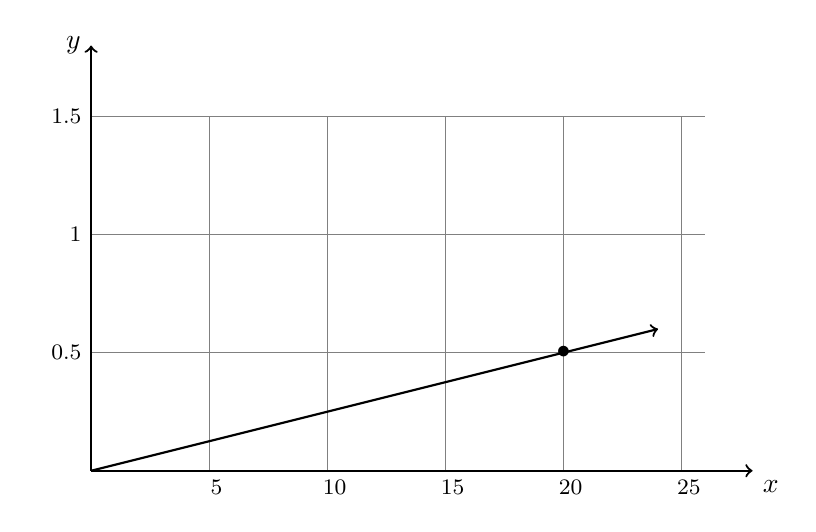
\begin{tikzpicture}[xscale=0.3, yscale=3]
    \draw [help lines, xstep=5, ystep=0.5] (0,0) grid (26,1.5);
    \draw [thick, ->] (0,0) -- (28,0) node [below right] {$x$};
    \foreach \x in {5,10,15,20,25}
      \draw[shift={(\x,0)},color=black] (0pt,0pt) -- (0pt,0pt) node[below] {\footnotesize \; $\x$};
    \draw [thick, ->] (0,0)--(0,1.8) node [left] {$y$};
    \foreach \y in {0.5, 1,1.5}
      \draw[shift={(0,\y)},color=black] (0pt,0pt) -- (0pt,0pt) node[left] {\footnotesize \; $\y$};
    \node at (20,0.5) {$\bullet$};
    %\draw [fill] (3,4) circle [radius=0.05] node[above right] {$B(3,4)$};
    \draw [->, thick] (0,0)--(24,0.6);
  \end{tikzpicture}
  \end{flushright}
\end{multicols}

\newpage  
\item Find the slope of the line $\overleftrightarrow{AB}$, $A(12,1)$, $B(44,5)$. Use the formula and show the substitution step. Express your result as a fraction, a decimal, and a percent grade.
\begin{multicols}{2}
  $\displaystyle m = \frac{y_B - y_A}{x_B - x_A}$
    \vspace{2cm}
    \begin{flushright}
      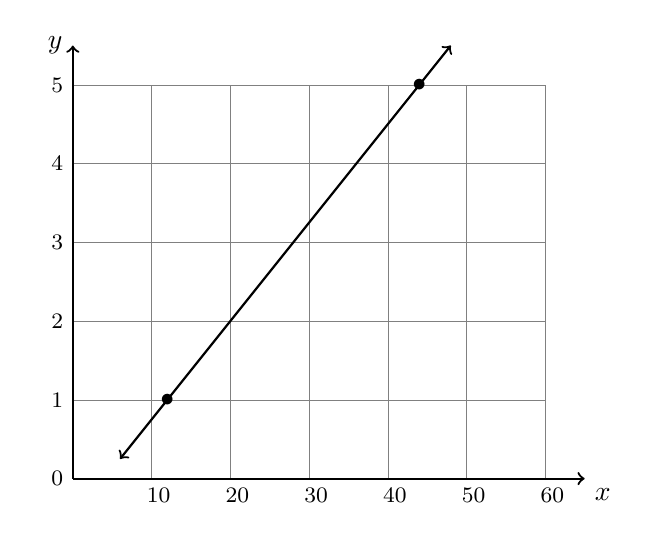
\begin{tikzpicture}[xscale=0.1, yscale=1]
        \draw [help lines, xstep=10, ystep=1] (0,0) grid (60,5);
        \draw [thick, ->] (0,0) -- (65,0) node [below right] {$x$};
        \foreach \x in {10,20,...,60}
          \draw[shift={(\x,0)},color=black] (0pt,0pt) -- (0pt,0pt) node[below] {\footnotesize \; $\x$};
        \draw [thick, ->] (0,0)--(0,5.5) node [left] {$y$};
        \foreach \y in {0,1,...,5}
          \draw[shift={(0,\y)},color=black] (0pt,0pt) -- (0pt,0pt) node[left] {\footnotesize \; $\y$};
        \node at (12,1) {$\bullet$};
        \node at (44,5) {$\bullet$};
        %\draw [fill] (3,4) circle [radius=0.05] node[above right] {$B(3,4)$};
        \draw [<->, thick] (6,0.25)--(48,5.5);
      \end{tikzpicture}\\
      \emph{Not to scale}
      \end{flushright}
    \end{multicols}

\newpage  
\item Find the equation of the line through the points $(0,2.4)$, $(70,3.8)$. Use the slope formula, then substitute the slope and $y$-intercept into a linear equation.
\begin{multicols}{2}
  $\displaystyle m = \frac{y_2 - y_1}{x_2 - x_1}$, \hspace{1cm} $y=mx+b$
  \columnbreak
  \begin{flushright}
    \emph{Not to scale}\\
    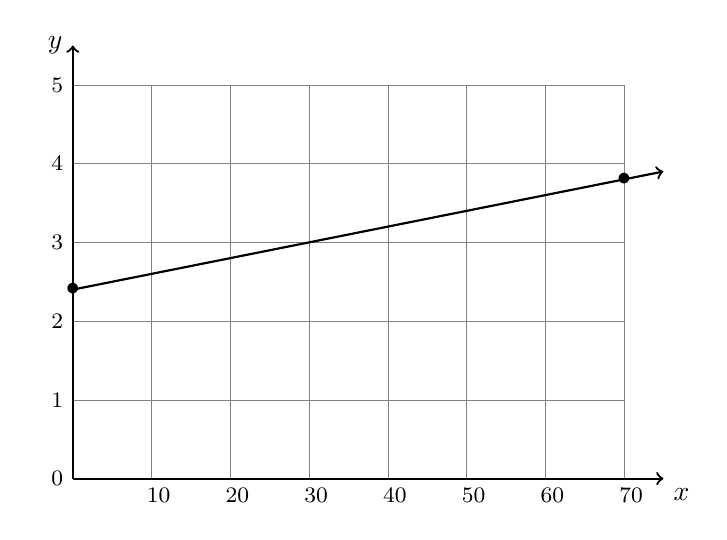
\begin{tikzpicture}[xscale=0.1, yscale=1]
      \draw [help lines, xstep=10, ystep=1] (0,0) grid (70,5);
      \draw [thick, ->] (0,0) -- (75,0) node [below right] {$x$};
      \foreach \x in {10,20,...,70}
        \draw[shift={(\x,0)},color=black] (0pt,0pt) -- (0pt,0pt) node[below] {\footnotesize \; $\x$};
      \draw [thick, ->] (0,0)--(0,5.5) node [left] {$y$};
      \foreach \y in {0,1,...,5}
        \draw[shift={(0,\y)},color=black] (0pt,0pt) -- (0pt,0pt) node[left] {\footnotesize \; $\y$};
      \node at (0,2.4) {$\bullet$};
      \node at (70,3.8) {$\bullet$};
      %\draw [fill] (3,4) circle [radius=0.05] node[above right] {$B(3,4)$};
      \draw [->, thick] (0,2.4)--(75,3.9);
    \end{tikzpicture}
    \end{flushright}
  \end{multicols}

\newpage
\item Complete each statement about linear equations.
\begin{enumerate}[itemsep=0.5cm]
  \item What is the $y$-intercept of the line $y = 1.25x - 13.5$?
  \item What is the percent grade of the line $\displaystyle y = 0.04x + 12.5$?
  \item What is the slope of a vertical line?
  \item What is the slope of the line $x=7$?

    \item If $m = 4$ then $m_{\perp}=$
    \item Lines $p$ and $q$ have slopes $m_p = -\frac{3}{2}$ then $m_q= +\frac{2}{3}$. Are they parallel, perpendicular, or neither? Justify your answer by showing the product of their slopes.
  \end{enumerate}

\newpage
\item Is the point $P(55,2.5)$ on the line: $y=0.012x+1.75$? \\[0.5cm]
Support your answer algebraically (substitute $P$'s coordinates into the equation).
\begin{flushright}
  \emph{Not to scale}\\
  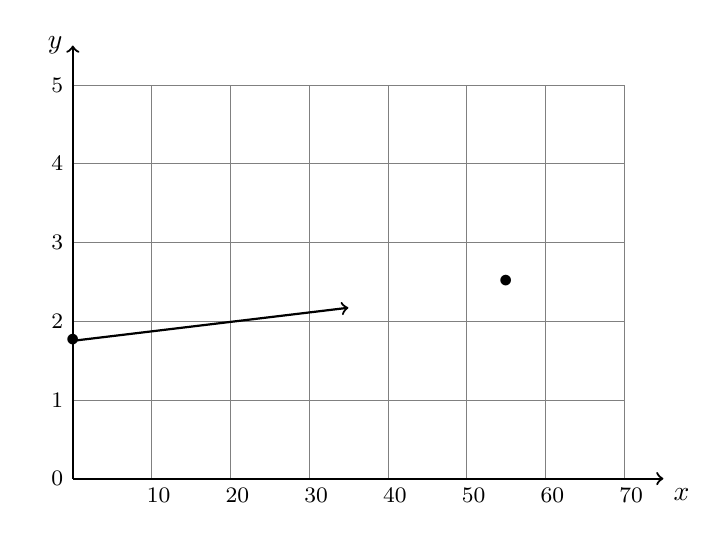
\begin{tikzpicture}[xscale=0.1, yscale=1]
    \draw [help lines, xstep=10, ystep=1] (0,0) grid (70,5);
    \draw [thick, ->] (0,0) -- (75,0) node [below right] {$x$};
    \foreach \x in {10,20,...,70}
      \draw[shift={(\x,0)},color=black] (0pt,0pt) -- (0pt,0pt) node[below] {\footnotesize \; $\x$};
    \draw [thick, ->] (0,0)--(0,5.5) node [left] {$y$};
    \foreach \y in {0,1,...,5}
      \draw[shift={(0,\y)},color=black] (0pt,0pt) -- (0pt,0pt) node[left] {\footnotesize \; $\y$};
    \node at (0,1.75) {$\bullet$};
    \node at (55,2.5) {$\bullet$};
    %\draw [fill] (3,4) circle [radius=0.05] node[above right] {$B(3,4)$};
    \draw [->, thick] (0,1.75)--(35,2.17);
  \end{tikzpicture}
  \end{flushright}

\newpage
\item Quadrilateral $ABCD$ with vertices $A(-2,5)$, $B(0,-1)$, $C(4,0)$, and $D(2,6)$ is shown. \\[0.5cm]
Find the slopes of each side. Is $ABCD$ a parallelogram? a rectangle? Justify your answer.
\begin{multicols}{2}
  Slope of $\overline{AB}=$\\[1.5cm]
  Slope of $\overline{BC}=$\\[1.5cm]
  Slope of $\overline{CD}=$\\[1.5cm]
  Slope of $\overline{AD}=$\\
  \begin{flushright}
    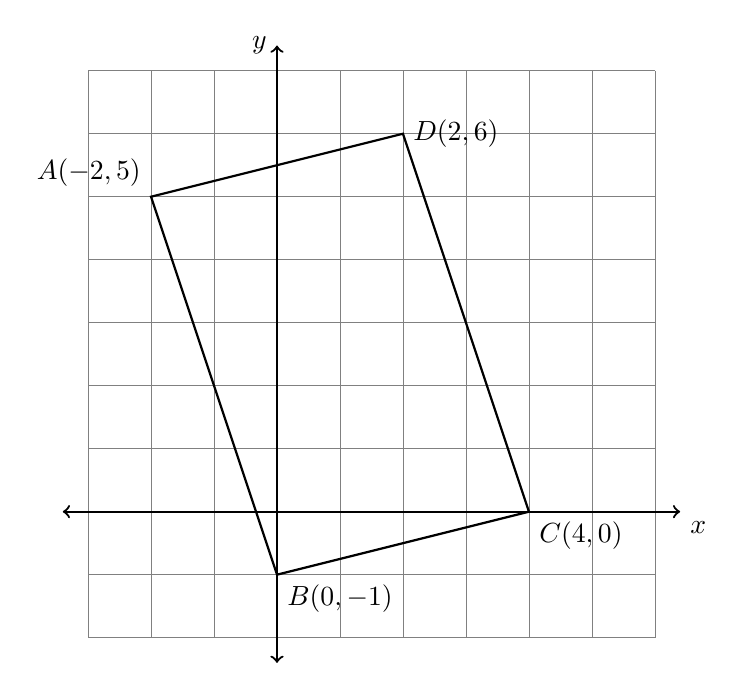
\begin{tikzpicture}[scale=0.8]
      \draw [help lines] (-3,-2) grid (6,7);
      \draw [thick, <->] (-3.4,0) -- (6.4,0) node [below right] {$x$};
      \draw [thick, <->] (0,-2.4)--(0,7.4) node [left] {$y$};
      \draw [thick] (-2,5) node[above left] {$A(-2,5)$}--
        (2,6) node[right] {$D(2,6)$}--
        (4,0) node[below right] {$C(4,0)$}--
        (0,-1) node[below right] {$B(0,-1)$}--
        cycle;
    \end{tikzpicture}
    \end{flushright}
  \end{multicols}

\newpage
\item Plot a parallelogram (not a rectangle) using Geogebra (use the grid). The legs must not be horizontal or vertical. Paste an image of your work in this Classkick slide from the clipboard or by using the ``camera'' tool.\\[0.25cm]
Spicy: Show the measures the slopes of the quadrilateral sides.

  
\newpage
\item 
    \begin{enumerate}
      \item Draw two sides $\overline{AD}$, $\overline{CD}$ to complete a parallelogram $ABCD$. \vspace{0.25cm}
      \item Write the slope of line $\overleftrightarrow{CD}$.
      \begin{multicols}{2}
        
      \item Write the equation of line $\overleftrightarrow{BC}$.\vspace{2cm}
      \item Is $\overleftrightarrow{CD} \perp \overleftrightarrow{BC}$? Show the product of their slopes is or is not $-1$.
    \begin{flushright}
      \includegraphics[width=9cm]{6-8 Slope-8.png}
    \end{flushright}
    Link: 
    https://www.geogebra.org/calculator/j8kx5ykf
\end{multicols}
\end{enumerate}


\end{enumerate}
\end{document}

\newpage
\item A point labeled $C$ and vector $(1,3)$ are shown Geogebra/classic. Identify the following objects and tools.
  \begin{enumerate}
    \item Circle the vector
    \item Make an ``X'' where to click for the menu ``Name \& Value'' that will label point $C$ as an ordered pair.
    \item Mark with an arrow the menu where the ``Translate by vector'' tool is found.
  \end{enumerate}
  \begin{flushright}
    \includegraphics[width=6in]{5-11Geogebra_toolbar.png}
  \end{flushright}
